
% $Header: /cvsroot/latex-beamer/latex-beamer/solutions/generic-talks/generic-ornate-15min-45min.en.tex,v 1.5 2007/01/28 20:48:23 tantau Exp $

\documentclass[smaller]{beamer}
\usepackage{booktabs}

\mode<presentation>
{
  \usetheme{Singapore}
  \usefonttheme[onlymath]{serif}
  % or ...
 %  \setbeamercovered{transparent}
  % or whatever (possibly just delete it)
}


\usepackage[czech]{babel}
% or whatever
\usepackage[utf8]{inputenc}

% or whatever
%\usepackage{times}
%\usepackage[T1]{fontenc}
% Or whatever. Note that the encoding and the font should match. If T1
% does not look nice, try deleting the line with the fontenc.


\title{PAS03 - random variables}

\author{Jan B\v rezina}
\institute % (optional, but mostly needed)
{
  %\inst{2}%
  Technical University of Liberec
}


% If you wish to uncover everything in a step-wise fashion, uncomment
% the following command: 

%\beamerdefaultoverlayspecification{<+->}

% ***************************************** SYMBOLS
\def\div{{\rm div}}
\def\Lapl{\Delta}
\def\grad{\nabla}
\def\supp{{\rm supp}}
\def\dist{{\rm dist}}
%\def\chset{\mathbbm{1}}
\def\chset{1}

\def\Tr{{\rm Tr}}
\def\sgn{{\rm sgn}}
\def\to{\rightarrow}
\def\weakto{\rightharpoonup}
\def\imbed{\hookrightarrow}
\def\cimbed{\subset\subset}
\def\range{{\mathcal R}}
\def\leprox{\lesssim}
\def\argdot{{\hspace{0.18em}\cdot\hspace{0.18em}}}
\def\Distr{{\mathcal D}}
\def\calK{{\mathcal K}}
\def\FromTo{|\rightarrow}
\def\convol{\star}
\def\impl{\Rightarrow}
\DeclareMathOperator*{\esslim}{esslim}
\DeclareMathOperator*{\esssup}{ess\,sup}
\DeclareMathOperator{\ess}{ess}
\DeclareMathOperator{\osc}{osc}
\DeclareMathOperator{\curl}{curl}

%\def\Ess{{\rm ess}}
%\def\Exp{{\rm exp}}
%\def\Implies{\Longrightarrow}
%\def\Equiv{\Longleftrightarrow}
% ****************************************** GENERAL MATH NOTATION
\def\Real{{\rm\bf R}}
\def\Rd{{{\rm\bf R}^{\rm 3}}}
\def\RN{{{\rm\bf R}^N}}
\def\D{{\mathbb D}}
\def\Nnum{{\mathbb N}}
\def\Measures{{\mathcal M}}
\def\d{\,{\rm d}}               % differential
\def\sdodt{\genfrac{}{}{}{1}{\rm d}{{\rm d}t}}
\def\dodt{\genfrac{}{}{}{}{\rm d}{{\rm d}t}}

\def\vc#1{\mathbf{\boldsymbol{#1}}}     % vector
\def\tn#1{{\mathbb{#1}}}    % tensor
\def\abs#1{\lvert#1\rvert}
\def\Abs#1{\bigl\lvert#1\bigr\rvert}
\def\bigabs#1{\bigl\lvert#1\bigr\rvert}
\def\Bigabs#1{\Big\lvert#1\Big\rvert}
\def\ABS#1{\left\lvert#1\right\rvert}
\def\norm#1{\bigl\Vert#1\bigr\Vert} %norm
\def\close#1{\overline{#1}}
\def\inter#1{#1^\circ}
\def\ol#1{\overline{#1}}
\def\ul#1{\underline{#1}}
\def\eqdef{\mathrel{\mathop:}=}     % defining equivalence
\def\where{\,|\,}                    % "where" separator in set's defs
\def\timeD#1{\dot{\overline{{#1}}}}

% ******************************************* USEFULL MACROS
\def\RomanEnum{\renewcommand{\labelenumi}{\rm (\roman{enumi})}}   % enumerate by roman numbers
\def\rf#1{(\ref{#1})}                                             % ref. shortcut
\def\prtl{\partial}                                        % partial deriv.
\def\Names#1{{\scshape #1}}
\def\rem#1{{\parskip=0cm\par!! {\sl\small #1} !!}}

\def\Xint#1{\mathchoice
{\XXint\displaystyle\textstyle{#1}}%
{\XXint\textstyle\scriptstyle{#1}}%
{\XXint\scriptstyle\scriptscriptstyle{#1}}%
{\XXint\scriptscriptstyle\scriptscriptstyle{#1}}%
\!\int}
\def\XXint#1#2#3{{\setbox0=\hbox{$#1{#2#3}{\int}$}
\vcenter{\hbox{$#2#3$}}\kern-.5\wd0}}
\def\ddashint{\Xint=}
\def\dashint{\Xint-}

% ******************************************* DOCUMENT NOTATIONS
% document specific
\def\rh{\varrho}
\def\vl{{\vc{u}}}
\def\th{\vartheta}
\def\vx{\vc{x}}
\def\vX{\vc{X}}
\def\vr{\vc{r}}
\def\veta{\vc{\eta}}
\def\dx{\,\d\vx}
\def\dt{\,\d t}
\def\bulk{\zeta}
\def\cS{\close{S}}
\def\eps{\varepsilon}
\def\phi{\varphi}
\def\Bog{{\mathcal B}}
\def\Riesz{{\mathcal R}}
\def\distr{\mathcal D}
\def\Item{$\bullet$}

\def\MEtst{\mathcal T}
%***************************************************************************
% highlight color
\setbeamercolor{my blue}{fg=blue}
\def\blue#1{{\usebeamercolor[fg]{my blue} #1}}

\setbeamercolor{my green}{fg=green}
\def\green#1{{\usebeamercolor[fg]{my green} #1}}

% color for term definition
\setbeamercolor{my orange}{fg=orange}
\def\df#1{{\usebeamercolor[fg]{my orange} #1}}
\def\xskip{{\vspace{2ex}}}

\def\cz#1{{\small (#1)}}

\begin{document}

\begin{frame}
  \titlepage
\end{frame}


\section{Random variable}
%
% TODO:
%  - distribution function for Alternative distribution
%  - example of calculation of EX a DX
%  - less about abstract probability space
%  - more about practical usage of DF and density ...


\begin{frame}{Probability space - abstraction}
\begin{itemize}
\item Consider survey asking people for: sex $S$, weight $W$, height $H$
\item has to consider probability space $\Omega = \Omega_{S} \times \Omega_{W} \times \Omega_{H}$
\item choice of the space depends on the variables we are observing\\
      ... unpractical  
\item probability space of "abstract events"
\item random variables as mappings from abstract space to the space of the variable
\end{itemize}
\end{frame}


\begin{frame}{Measurement as random variable}
\blue{Probability space:} 
$\Omega$ \dots set of all possible humans
$\mathcal S$ \dots a system of subsets
$p$ \dots probability measure

\xskip
\blue{mapping:} mesurement, observation

\xskip
\blue{Random variable}:
sex, weight, height

\end{frame}



\begin{frame}{Random variable}
Random variable is mapping from probability space into $\Real$,\\
it forms a probability space on $\Real$.
\vspace{2ex}
\begin{center}
 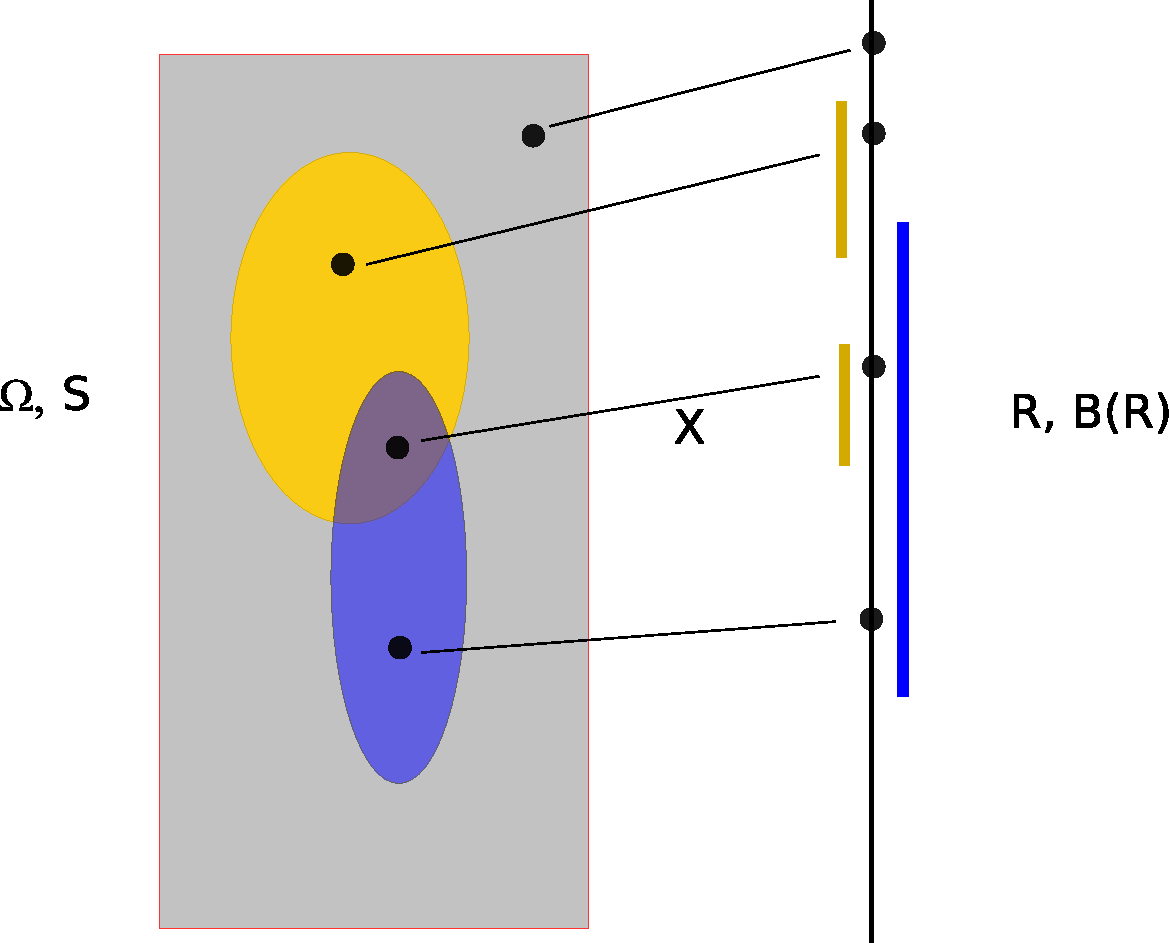
\includegraphics[scale=0.4]{03_nv.pdf}
\end{center}
\end{frame}


\begin{frame}{Definition of random variable}
\begin{definition}
 Let $\mathcal P=(\Omega, \mathcal S, P)$ be a probability space.\\
 Then \df{random variable} \cz{náhodná veličina} is a mapping $X: \Omega \to \Real$,\\
 such that counter-image of any measurable set (Borel set $B \in \mathcal B(R)$)\\
 is measurable in $\mathcal P$, i.e. ($X^{-1}(B) \in \mathcal S$).\\
 We can also say, that random variable is a \df{measurable function} .
\end{definition}

\xskip
RV maps the probability space $\mathcal P$ to the space $(\Real, \mathcal B, \tilde P)$.\\

\xskip
RV is uniquely given by the \df{distribution function} (DF)
\[
   F_X(x) = \tilde P(X(\omega) \le x) = P( X^{-1}\big(  (-\infty, x] \big)
\]
Further we shall not distinguish  $\tilde P$ and $P$.
\end{frame}

\begin{frame}{Distribution function}
\blue{Properties of DF:}
\begin{enumerate}
 \item $0\le F(x) \le 1$
 \item $F$  is non-decreasing
 \item \[
  \lim_{x\to -\infty} F(x) = 0,\quad \lim_{x\to \infty} F(x) = 1
\]
 \item continuous from the right 
\end{enumerate}

\xskip

Contrarily, every DF determines a random variable: 
\begin{theorem}
  For every function $F$ with properties $1-4$, there exists random variable $X$, such that $F$ is its distribution function.
\end{theorem}
\end{frame}


\begin{frame}{ECDF}
\blue{Empirical (Cumulative) Distribution Function}\\
\cz{Empirická distribuční funkce}

\xskip
Plots estimates of probabilities of events $\{ X \le x\}$\\
as relative frequency of data smaller then $x$.

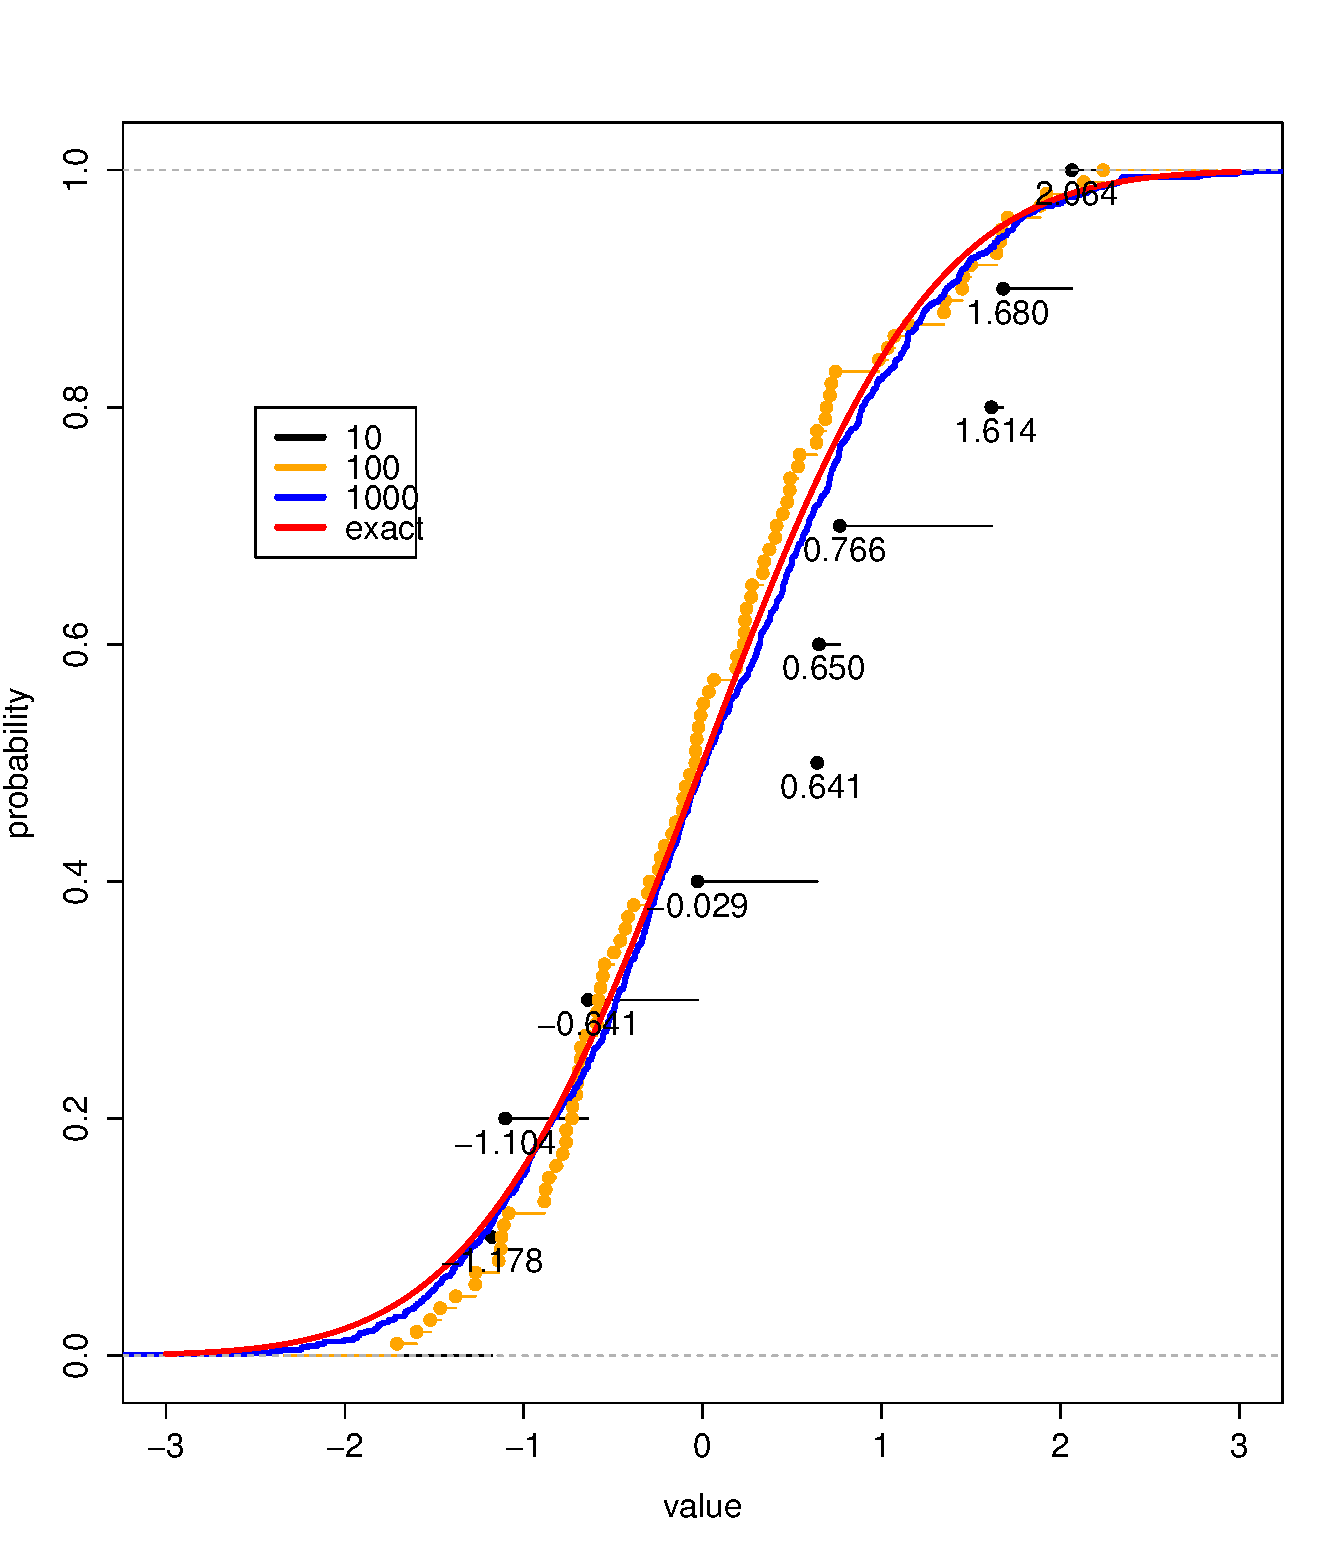
\includegraphics[scale=0.25]{01_ecdf.pdf}
\end{frame}


\begin{frame}{Discrete distribution}

\df{Discrete random variable}\\

\begin{itemize}
\item RV $X$ with finite or countable image
\item consists from values $x_i$ with probabilities $p_i$,
\item $\sum_i p_i =1$.\\
\item it distribution function is piecewise constant, with jumps of height $p_i$ in points $x_i$.
\end{itemize}
\end{frame}


\begin{frame}{Examples}
Alternative distribution, 
\[
    P(X=0)=a,\quad  P(X=1)=1-a 
\]
Binomial distribution, 
\[
    P(X=k) = \binom{n}{k} a^{k} (1-a)^{n-k} 
\]
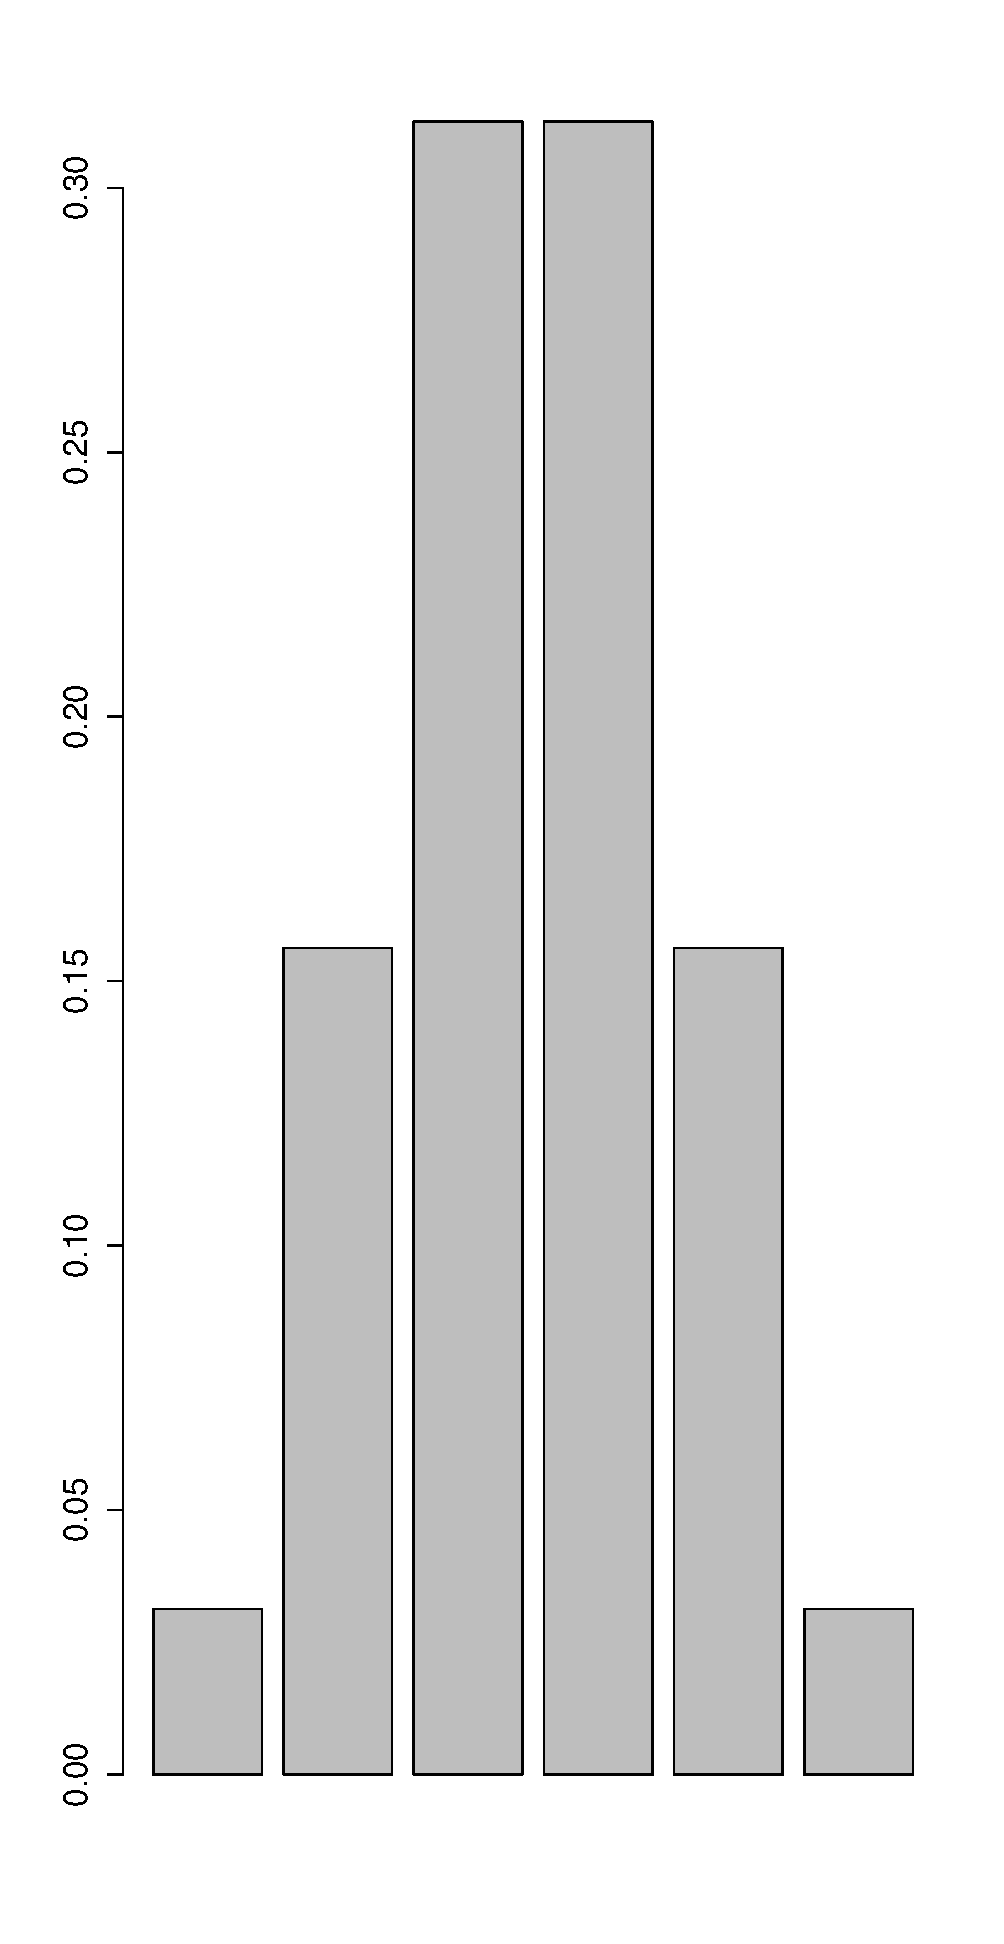
\includegraphics[keepaspectratio=false,width=8cm,height=4cm]{03_binom_hist.pdf}
\end{frame}


\begin{frame}{Continuous distribution}
\xskip
\df{Continuous random variable}\\
\dots if there exists a non-negative function $f_X$ such that:
\[
   F_X(x) = \int_{-\infty}^x f_X(t) \dt
\]
$f_X$ is called \df{probability density}\cz{hustota pravděpodobnosti} and it holds $\int_{-\infty}^{\infty} f_X(x) = 1$.

\xskip
Remark: Continuous RV has continuous DF.
\end{frame}


\begin{frame}{Examples}
\blue{Continuous random variable}\\
Normal distribution
\[
    f(x) = \frac{1}{\sqrt{2\pi \sigma^2}} exp\Big( - \frac{ (x - \mu)^2}{2\sigma^2} \Big)
\]
\end{frame}


\begin{frame}{Expectation \cz{střední hodnota}}
for \blue{discrete} random variable $X$:
\[
  EX = \sum_i x_i P(X = x_i) = \sum_i x_i p_i
\]
for \blue{continuous} random variable $X$:
\[
  EX = \int_{-\infty}^{+\infty} xf_X(x) \d x
\]

\xskip
it may not exist, e.g. $x_i = 2^n$, $p_i = 2^{-n}$ or $f(x)=\frac{1}{1+x^2}$\\

\xskip
linearity: $E(aX+bY) = aEX + bEY$
\end{frame}
\begin{frame}{Law of the unconsious statistician}
expectation of \blue{transformed RV} $Y = h(X)$: 
\[
 EY =  E y(X) = \int_{-\infty}^{+\infty} y(x) f_X(x) \d x
\]
For discrete case it is clear:
\[
   EY = \sum_i y_i p_i = \sum_i y(x_i) p_i
\]


Similarly for continuous case, use same probability diferencials:
\[
   f_Y(y) \d y = \d F_Y(y(x)) = \d F_X(x) = f_X(x) \d x
\]
Thus
\[
   EY = \int_{-\infty}^{+\infty} y f_Y(y) \d y = \int_{-\infty}^{+\infty} y(x) f_X(x) \d x
\]
\end{frame}

\begin{frame}{Example of calculation}

\end{frame}


\begin{frame}{Moments}
\df{$r$th-moment}:
\[
 \mu'_r(X) = E(X^r)
\]
\df{$r$th-central moment}: 
\[
 \mu_r(X) = E\big([X - EX]^r\big)
\] 
\df{variance}: $DX$, $\sigma^2$, $var(X)$: 
\begin{multline*}
  \mu_2(X) = DX = E( (X-EX)^2 ) = \\
E( X^2 + (EX)^2 - 2X EX) = E(X^2) - (EX)^2 = \mu'_2 - (\mu'_1)^2
\end{multline*}
\df{standard deviation}: $\sigma = \sqrt{\sigma^2}$\\
skewness: $\alpha_3 = \mu_3/\sigma^3$\\
kurtosis: $\alpha_4 = \mu_4/\sigma^4 -3$
\end{frame}

\begin{frame}{Quantiles}
For given $\alpha \in (0,1)$ find $x$ such that $P(X < x) = \alpha$. \\
\df{ Quantile function}:
\[
  F^{-1}(\alpha) = \inf\{x \where F_X(x)\ge\alpha\}
\]
\blue{notation}: $x_\alpha$, $u_\alpha$; quantile on level $\alpha$, $\alpha$-quantile,
median $x_{0.5}$, quartiles,\dots

 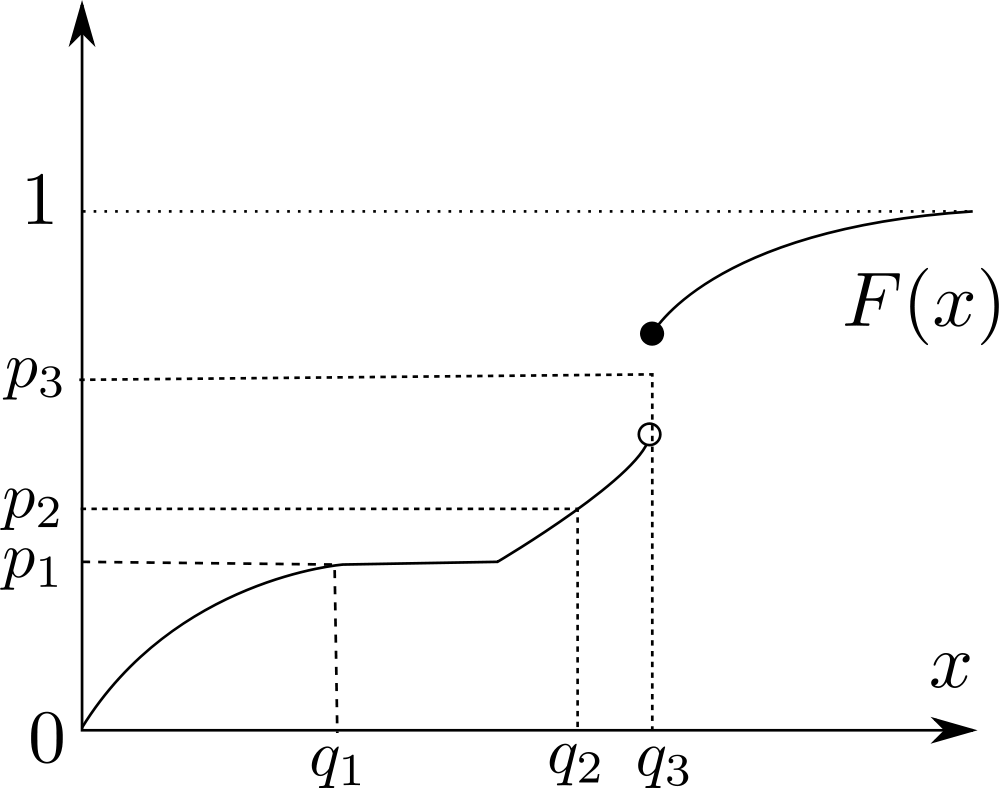
\includegraphics[scale=0.2]{./03_quantile_distribution_function.png}
 % 03_quantile_distribution_function.png: 1000x788 pixel, 72dpi, 35.28x27.80 cm, bb=0 0 1000 788
\end{frame}

\begin{frame}{Sample approximations}
\begin{tabular}{ll}
\toprule
Exact & Sample \\
\midrule
distribution function  &        ECDF \\
 & \\
EX                     &        sample mean  \\
$\sum_{k} x_k p(x_k)$  &        $\ol{X}=\sum_{i} X_i / n$ \\
$\int_\Real x f(x)$    &          \\      
 & \\
variance               &        sample variance \\
$\sum_{k} (x_k - EX)^2 p(x_k)$  &  $ \frac{1}{n-1} \sum_{i} (X_i - \ol{X})^2 $\\
$\int_\Real (x- EX)^2 f(x) $   &  \\  
\bottomrule
\end{tabular}
\end{frame}

\end{document}


